\section{Attribute Definition}
\textcolor{red}{Throughout this section we will define the indicators.}

\subsection{Technical parameters}

\paragraph{Thermal efficiency} indicates the fraction of thermal power generated by fission that is converted into net electrical power, accounting for in-plant consumption. Efficiency values were calculated using net electrical power output and thermal power data from the ARIS database \cite{iaea2025aris}:
$$
\eta = \frac{P_{el,net}}{P_{th}}
$$

\begin{table}[!ht]
    \centering
    \begin{tabularx}{\textwidth}{X c}
        \toprule
        \textbf{Reactor Model} & \textbf{Net Efficiency [\%]} \\
        \midrule
        APR1400         & 35.2 \\
        EPR 1750        & 36.2 \\
        AP1000          & 32.4 \\
        BWRX-300        & 34.5 \\
        Rolls Royce SMR & 34.6 \\
        NuScale         & 30.8 \\
        \bottomrule
    \end{tabularx}
    \caption{Net electrical efficiencies for selected reactor models}
    \label{tab:reactor-efficiency}
\end{table}


\paragraph{Discharge Burnup} measures the energy extracted per unit of heavy metal fuel ($MWd/tonHM$). Data for APR1400 and AP1000 were sourced from the ARIS database \cite{iaea2025aris}, while EPR 1750 data were obtained from \cite{NRC_ML052280170}. Ranges are provided for SMRs due to design variability.

\begin{table}[!ht]
    \centering
    \begin{tabularx}{\textwidth}{X c}
        \toprule
        \textbf{Reactor Model} & \textbf{Discharge Burnup [$MWd/tonHM$]} \\
        \midrule
        APR1400         & 46.5 \\
        EPR 1750        & 55 \\
        AP1000          & 50 \\
        BWRX-300        & $50 \pm 5$ \\
        Rolls Royce SMR & $55 \pm 5$ \\
        NuScale         & $52.5 \pm 2.5$ \\
        \bottomrule
    \end{tabularx}
    \caption{Discharge burnup for selected reactor models}
    \label{tab:reactor-burnup}
\end{table}



\paragraph{\gls{mox}} fuel is produced through spent nuclear fuel reprocessing and offers a solution for partially closing the nuclear fuel cycle in thermal reactors. While this process generates some secondary waste, it provides several strategic advantages: reducing final nuclear waste volumes, minimizing mining waste, and decreasing dependence on uranium imports. The latter is particularly relevant for Europe, which lacks significant domestic uranium deposits. However, reprocessing also presents proliferation risks since the extracted plutonium could potentially be diverted for weapons production. Due to these competing factors, nuclear fuel reprocessing is a fundamental strategic decision; the United States has foregone this practice, while France and UK have implemented the process in their nuclear programs \cite{CRS_Reprocessing_Spent_Fuel_2025}.

Given the European context of this study, MOX compatibility is considered a relevant reactor attribute. The evaluation methodology assigned each reactor design an initial score (0-10) based on its maximum MOX core fraction capability, followed by qualitative adjustments reflecting design-specific features. The complete scoring process and results are detailed in Table \ref{tab:mox-compatibility}.

\begin{table}[!hb]
    \centering
    \begin{tabularx}{\textwidth}{l c X c c}
        \toprule
        \textbf{Reactor Model} & \textbf{MOX[\%]} & \textbf{Considerations} & \textbf{Score} & Sources \\
        \midrule
        APR1400         & 33 & - & 3/10 & \cite{iaea2025aris} \\
        \cmidrule(lr){1-5}
        EPR 1750        & 100 & 50\% without modifications, to reach 100\% "design adaptations which are not significantly costly" are required.  & 9/10 & \cite{iaea2025aris, osti_22257897} \\
        \cmidrule(lr){1-5}
        AP1000          & 50 & 50\% without modification, to reach 100\% major modifications are required & 6/10 & \cite{iaea2025aris, FETTERMAN2009324} \\
        \cmidrule(lr){1-5}
        BWRX-300        & 0 & GNF-2 Not manufactured with MOX & 0/10 & \cite{CNSC_BWRX300_Fuel_Design} \\
        \cmidrule(lr){1-5}
        Rolls Royce SMR & 0 & Rolls Royce states that they are not planning to use MOX & 0/10 & \cite{RollsRoyce_SMR_GDA_Consultation} \\
        \cmidrule(lr){1-5}
        NuScale         & 0 & Not licensing for MOX but a study reveals support is possible without design modifications & 1/10 & \cite{NRC_ML17007A001, NuScale_MOX_2016} \\
        \bottomrule
    \end{tabularx}
    \caption{MOX fuel compatibility scores and maximum MOX fraction}
    \label{tab:mox-compatibility}
\end{table}

\paragraph{Technological Readiness} of each reactor design was assessed by expert consultation by presenting them ... and ...

\subsection{System parameters}
\paragraph{Net Electric Power Output} 
\begin{table}[!ht]
    \centering
    \begin{tabularx}{\textwidth}{l X X}
        \toprule
        \textbf{Reactor Model} & \textbf{Net Power Output $[MW_{e,net}]$} & Data Source\\
        \midrule
        APR1400         & 1340 & \cite{IAEA_PRIS_2025} \\
        EPR 1750        & 1630 & \cite{IAEA_PRIS_2025} \\
        AP1000          & 1120 & \cite{IAEA_PRIS_2025} \\
        BWRX-300        & 300 & \cite{iaea2025aris} \\
        Rolls Royce SMR & 470 & \cite{iaea2025aris} \\
        NuScale         & 77 (per unit) & \cite{iaea2025aris} \\
        \bottomrule
    \end{tabularx}
    \caption{Load following capabilities and power output}
    \label{tab:load-power_output}
\end{table}

\paragraph{\glspl{lfc}} can be quantitatively assessed using characteristic curves that represent ramp-up and ramp-down rates as a function of load (expressed as percentage of nominal power $\%P_{nom}$), as illustrated in Figure \ref{fig:load-following-curve}. To facilitate comparative analysis, these performance curves are reduced to scalar values through integration of the area under said curve.

For benchmarking purposes, \glspl{lfc} were calculated for two modern gas turbine configurations: A heavy-duty combined cycle plant featuring two GE Vernova 9HA.02 gas turbines (2015 data) \cite{GE_9HA_Gas_Turbine_2015} and an equivalent plant configuration utilizing aeroderivative GE LM2500XPRESS+G5 DLE UPT gas turbines (2025 data) \cite{GEVernova_LM2500XPRESS_2025}. Hydroelectric plants are also included as a reference for the highest flexibility, a 1989 publication by the US Office of Technology Assessment \cite{OTA_Electric_Power_Wheeling_1989} reports that the response rate of large (>60MW) hydroelectric plants ranges from 4 to 6 \%P$_{nom}$/s, which translates to 240 to 360 \%P$_{nom}$/min. A graph from a 1994 conference reported in a technical analysis from 2009 shows that some hydro plant can achieve 0 to 100\% in much less then a minute and from black startup to full power in around 5 minutes For the comparison we indicate greater then 100\%. \cite{osti_219975, MWH_Pumped_Storage_Wind_2009}

To establish an upper benchmark hydroelectric plants were included in the comparative analysis. A 1989 U.S. Office of Technology Assessment report \cite{OTA_Electric_Power_Wheeling_1989} documents that large (>60 MW) hydroelectric facilities demonstrate remarkable load-following capabilities, with response rates ranging from 4 to 6 \%P$_{nom}$/s (equivalent to 240-360 \%P$_{nom}$/min). Additional performance data from a 1994 conference presentation, cited in a 2009 technical analysis \cite{osti_219975, MWH_Pumped_Storage_Wind_2009}, indicates that certain hydroelectric installations can achieve 0-100\% load changes in under one minute and black start to full power operation in approximately five minutes. For the purposes of this comparison, hydroelectric flexibility is conservatively represented as >100 \%P$_{nom}$/min.

The results of these analyses are presented in Table \ref{tab:load-following-capabilities}.

\begin{figure}[!hb]
    \centering
    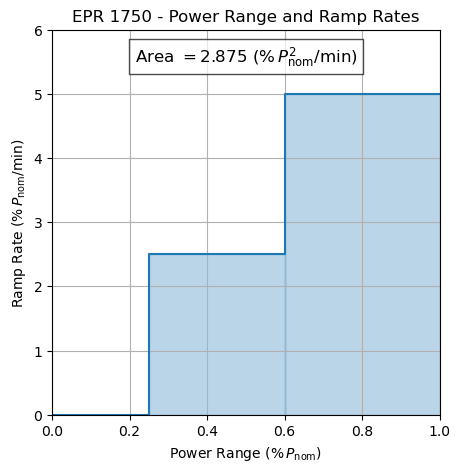
\includegraphics[width=0.7\textwidth]{imgs/load_following_curve.png}
    \caption{Example \gls{lfc} curve for EPR-1750}
    \label{fig:load-following-curve}
\end{figure}

\begin{table}[!hb]
    \centering
    \begin{tabularx}{\textwidth}{l X X}
        \toprule
        \textbf{Reactor Model} & \textbf{\gls{lfc} $\left[ \frac{\%P_{nom}^2}{min} \right]$} & Data Source \\
        \midrule
        APR1400         & 0.21  & \cite{iaea2025aris} \\
        EPR 1750        & 2.88 & \cite{OECD_NEA_Load_Following_2011} \\
        AP1000          & 4.25  & \cite{iaea2025aris} \\
        BWRX-300        & 0.25  & \cite{iaea2025aris} \\
        Rolls Royce SMR & 2.00 & \cite{iaea2025aris} \\
        NuScale         & 2.00   & \cite{ENCO_SMR_Analysis_2022} \\
        GE 9HA.02 2xCC & 7.02 & \cite{GE_9HA_Gas_Turbine_2015} \\
        GE LM2500XPRESS+G5 2xCC & 40.54 & \cite{GEVernova_LM2500XPRESS_2025} \\
        Hydroelectric   & >100 & \cite{OTA_Electric_Power_Wheeling_1989, osti_219975, MWH_Pumped_Storage_Wind_2009} \\
        \bottomrule
    \end{tabularx}
    \caption{Load following capabilities and power output}
    \label{tab:load-following-capabilities}
\end{table}

\subsection{Economic Indicators}

\paragraph{Capital Costs} are capital costs...

\begin{table}[!hb]
    \centering
    \begin{tabularx}{\textwidth}{X X X}
        \toprule
        \textbf{Option} & \textbf{PROs} & \textbf{CONs}\\
        \midrule
        Use NOAK estimates          & Use of estimates in all cases, comparable values & It's not realistic and not fair towards more mature designs \\
        \cmidrule(lr){1-3}
        Use FOAK estimates/data        & Better data for three large reactors & We are mixing up real data and estimates \\
        \cmidrule(lr){1-3}
        Use NOAK and apply FOAK-to-NOAK conversion         & Comparable values, with awareness of current know-how & rely on a model \\
        \cmidrule(lr){1-3}
        Present NOAK and FOAK to experts along with technological readiness overview and let them evaluate &  As before & rely on expert judgment \\
        \bottomrule
    \end{tabularx}
    \caption{Options overview}
    % \label{tab:operational-costs}
\end{table}

The same applies to commissioning time.

It is important to note that these costs refer to an Nth of a kind installation and will not be representative of the FOAK costs. Moreover as detailed by Rothwell 2022 \cite{ROTHWELL2022112905} the costs of recent nuclear installations in Europe and the US have been significantly higher than those announced at the start of the project. For this reason we will apply a FOAK-to-NOAK factor to better represent the real costs. For example the EPR-1600 announced costs for Flamanville-3 was 1886 $USD_{2020}/kW_e$ but have risen to 8600 $USD_{2020}/kW_e$ \cite{NEA2020}. All Values are summarized in Table \ref{tab:capital-costs}. \\

For reference, the capital costs of the same plants as the previous section have been reported by the US Energy Information Administration \cite{EIA_Capital_Costs_AEO2024}.

We want to clarify that the data has all been converted to 2020 USD since the main source of data \cite{STEIGERWALD2023128204} and \cite{NEA2020} reports all costs in this currency and year. \\

\begin{table}[!hb]
    \centering
    \begin{tabularx}{\textwidth}{l X X X}
        \toprule
        \textbf{Reactor Model} & \textbf{Capital Cost of NOAK [\$/kWe]} & \textbf{Capital Cost of FOAK [\$/kWe]} & Data Source \\
        \midrule
        APR-1400         & 1828 & 2410 & \cite{STEIGERWALD2023128204, NEA2020} \\
        EPR-1750        & 2150 & 8600 & \cite{STEIGERWALD2023128204, NEA2020} \\
        AP-1000          & 2000 & 8600 & \cite{STEIGERWALD2023128204, NEA2020} \\
        BWRX-300        & 2318 & 3467 & \cite{ReutersEvents2018} \\
        Rolls Royce SMR & 6050 & 7408 & \cite{PowerTechnology2022} \\
        NuScale         & 2850 & 3600 & \cite{NuScale2020} \\
        \textbf{Other Power Plants} & & & \\
        Onshore Wind   & - & 1265 & \cite{EIA_Capital_Costs_AEO2024} \\
        Solar PV + Battery & - & 2175 & \cite{EIA_Capital_Costs_AEO2024} \\
        Hydroelectric  & - & 6007 & \cite{EIA_Capital_Costs_AEO2024} \\
        \bottomrule
    \end{tabularx}
    \caption{Capital costs for selected reactor models}
    \label{tab:capital-costs}
\end{table}

\paragraph{Commissioning Time} see observations in the previous section.

I would apply a +0.5 years to planned commissioning time on the APR and AP based on the planned commissioning time of the EPR that differs by 0.5 between UK and Chinese plannings. 

\begin{table}[!hb]
    \centering
    \begin{tabularx}{\textwidth}{l X X c}
        \toprule
        \textbf{Reactor Model} & \textbf{Planned Commissioning Time} & \textbf{Last unit Commissioning Time} & Data Source\\
        \midrule
        APR1400         & 5.0 in Korea & 10 and 8 in Korea & \cite{nea2020unlocking} \\
        EPR 1750        & 5.0 in Europe, 4.5 in China & 9 in Taishan, 17 in Flamanville and Olkiluoto & \cite{nea2020unlocking} \\
        AP1000          & 5.0 in USA & 9 in Sanmen, 10 and 11 at Vogtle & \cite{nea2020unlocking} \\
        BWRX-300        & 2 $\sim$ 3 & NA & \cite{GEVernova_Nuclear_2025} \\
        Rolls Royce SMR & 4.0 & NA & \cite{RollsRoyce_SMR_Approach_2025} \\
        NuScale         & 3.0 & NA & \cite{NuScale_Power_Module_2025} \\
        \bottomrule
    \end{tabularx}
    \caption{Technological readiness and planned commissioning time}
    \label{tab:tech-readiness}
\end{table}


\paragraph{Operational Costs} are costs due to operations...

Steigerwald et al. (2023) \cite{STEIGERWALD2023128204} provides comprehensive cost analyses for future nuclear installations, including capital and operational expenditures for both SMRs and large reactors. The study reports operational costs in $USD_{2020}/MWh_e$ for EPR and APR1400 designs, as well as a "Long-Term US" category which this analysis uses as AP1000 costs. For SMRs, operational costs were originally presented in power-based units ($USD_{2020}/MW_e$), requiring conversion to energy-based measurements ($USD_{2020}/MWh_e$) using a Gaussian distribution of capacity factors ($\mu$ = 90\%, $\sigma$ = 5\%) according to:

$$
\frac{USD_{2020}}{MWh_e} = \frac{USD_{2020}}{MW_e} \cdot \frac{1}{CF \cdot 8760 \frac{h}{year}}
$$

The same study reports fuel costs of $6.23 USD_{2020}/MWh_e$ for PWR-based technologies with the exceptions of NuScale at $7.15 USD_{2020}/MWh_e$ and the only BWR reactor at $29.55 USD_{2020}/MWh_e$. For comparative context, operational cost estimates for utility-scale onshore wind, hydroelectric, and solar PV (with single axis tracking and DC battery storage) were obtained from the U.S. Energy Information Administration \cite{EIA_Capital_Costs_AEO2024}. All cost data have been standardized to 2020 USD to maintain consistency with the primary data sources \cite{STEIGERWALD2023128204, NEA2020}, values are presented in Table \ref{tab:operational-costs}.


\begin{table}[!hb]
    \centering
    \begin{tabularx}{\textwidth}{l X X}
        \toprule
        \textbf{Reactor Model} & \textbf{Operative Cost [\$/MWh]} & Data Source\\
        \midrule
        APR-1400          & 18.44 & \cite{STEIGERWALD2023128204} \\
        EPR-1750        & 14.26 & \cite{STEIGERWALD2023128204} \\
        AP-1000          & 18.69 & \cite{STEIGERWALD2023128204} \\
        BWRX-300        & $18.30 \pm 0.82$ & \cite{STEIGERWALD2023128204} \\
        Rolls Royce SMR & $65.68 \pm 2.94$ & \cite{STEIGERWALD2023128204} \\
        NuScale         & $22.76 \pm 1.02$ & \cite{STEIGERWALD2023128204} \\
        \textbf{Other Power Plants} & & \\
        Onshore Wind   & 28.08 & \cite{EIA_Capital_Costs_AEO2024} \\
        Solar PV + Battery & 33.33 & \cite{EIA_Capital_Costs_AEO2024} \\
        Hydroelectric  & 28.49 & \cite{EIA_Capital_Costs_AEO2024} \\
        \bottomrule
    \end{tabularx}
    \caption{Economic costs for selected reactor models}
    \label{tab:operational-costs}
\end{table}


\paragraph{Potential Impact on the energy market} can be estiated by...

\subsection{Indicators on Social Matters}
\paragraph{Potential Reduction of \glspl{ghg}} were quantified by comparing each country's 2024 emissions against projected emissions following deployment of one reactor unit. Country-specific GHG emission intensities were derived from Electricity Maps aggregated data \cite{ElectricityMaps_CarbonIntensity_2024}. Total load were obtained from the ENTSO-E Transparency Platform \cite{ENTSOE_Transparency_2025}. Due to non-normal data distributions, median values with interquartile ranges were employed to characterize uncertainty (Table~\ref{tab:ghg-intensity-country}). \\

\begin{table}[!ht]
    \centering
    \begin{tabularx}{\textwidth}{l c c c}
        \toprule
        Country / Region & Annual Load [TWh] & GHG intensity [gCO$_2$-eq/kWh] & Total annual GHG [MtCO$_2$-eq/yr] \\
        \midrule
        Italy (IT)        & draft & 240 & 72.0 \\
        Switzerland (CH)  & 60  & draft  & 1.8 \\
        Poland (PL)       & 160 & 700 & draft \\
        France (FR)       & 460 & draft  & 23.0 \\
        \bottomrule
    \end{tabularx}
    \caption{Country-level electricity load, grid GHG intensity and total annual GHG emissions. (Total = Load [TWh] * intensity [gCO$_2$-eq/kWh] / 1000)}
    \label{tab:ghg-intensity-country}
\end{table}

For nuclear generation's lifecycle emissions, Liu et al.'s (2023) comprehensive meta-analysis of 42 studies \cite{10.3389/fenrg.2023.1147016} served as the primary reference, reporting a global average of $15.815 \pm 3.59 \; gCO_{2,\text{eq}}/kWh_e$ for light water reactors. This conservative estimate was selected despite lower values observed in specific contexts: French nuclear operations typically range between $ 2 \sim 6 \; gCO_{2,\text{eq}}/kWh_e$ according to both operational data \cite{paillere_2021} and IAEA assessments \cite{IAEA_Climate_Change_Nuclear_Power_2022}, while individual studies on french reactors have reported values as high as $12 \; gCO_{2,\text{eq}}/kWh_e$ \cite{paillere_2021}. The global average was preferred to account for potential regional variations in fuel cycle practices and construction impacts. \\

Small modular reactors (SMRs) were assigned an emission intensity of $17.24 \pm 3.91$ $gCO_{2,\text{eq}}/kWh_e$, incorporating Carless et al.'s (2016) finding that SMRs exhibit approximately $9\%$ higher lifecycle emissions than conventional large LWRs due to reduced economies of scale in construction and fuel production \cite{CARLESS201684}. \\

The GHG reduction benefit was calculated as the percentage improvement between current energy mixes $GHG_{current\ mix}$  and the nuclear deployment scenario $GHG_{nuclear}$:
$$
GHG_{Benefit} (\%) = \left(1 - \frac{GHG_{nuclear}}{GHG_{current\ mix}}\right) \times 100
$$

% The results are shown in Table \ref{tab:ghg-benefit-country}.
% \begin{table}[!ht]
%     \centering
%     \begin{tabularx}{0.7\textwidth}{l c c}
%         \toprule
%         \textbf{Country/Region} & \textbf{GHG Reduction (Large) [tCO2/MWh]} & \textbf{GHG Reduction (SMR) [tCO2/MWh]} \\
%         \midrule
%         Italy (IT)        & 0.85 & 0.83 \\
%         Switzerland (CH)  & 0.10 & 0.09 \\
%         Poland (PO)       & 0.90 & 0.88 \\
%         France (FR)       & 0.15 & 0.14 \\
%         \bottomrule
%     \end{tabularx}
%     \caption{GHG emission intensity benefit by country for large reactors and SMRs}
%     \label{tab:ghg-benefit-country}
% \end{table}
\paragraph{Spent Nuclear Fuel Production} was estimated based on...

\paragraph{Mining Waste} are estimated ....

\paragraph{Percived Safety} is an important point ...
